%=================================================================
\section{Introduction}\label{sec-intro}

Bike sharing systems are a means of renting bicycles where the process of obtaining membership, rental, and bike return is automated via a network of kiosk locations throughout a city. Using these systems, people are able rent a bike from a one location and return it to a different place on an as-needed basis. Currently, there are over 500 bike-sharing programs around the world.

The data generated by these systems makes them attractive for researchers because the duration of travel, departure location, arrival location, and time elapsed is explicitly recorded. Bike sharing systems therefore function as a sensor network, which can be used for studying mobility in a city. In this competition, participants are asked to combine historical usage patterns with weather data in order to forecast bike rental demand in the Capital Bikeshare program in Washington, D.C.


\section{Dataset Description} \label{sec-preliminaries}

\begin{itemize}
  \item
  %\emph{Group Outlying Aspects Mining}
  The competition provides hourly rental data spanning two years. For this competition, the training set is comprised of the first 19 days of each month, while the test set is the 20th to the end of the month. You must predict the total count of bikes rented during each hour covered by the test set, using only information available prior to the rental period.

  \item
  Data Fields
  \end{itemize} 
    
  \bigskip 
    \begin{tabular}{ l | l }
      \toprule
      Attribute     &  Description          \\
      \midrule
      datetime       &  hourly date + timestamp  \\
      season      & 1 = spring, 2 = summer, 3 = fall, 4 = winter\\ 
      holiday  & whether the day is considered a holiday\\
      workingday & whether the day is neither a weekend nor holiday\\
      weather    & 1: Clear,2: Mist, 3: Light Snow, Light Rain , 4: Extreme weather\\ 
      temp  & temperature in Celsius\\
      atemp  & "feels like" temperature in Celsius\\
      humidity  & relative humidity\\
      windspeed  &  wind speed\\
      casual  & number of non-registered user rentals initiated\\
      registered  & number of registered user rentals initiated\\
      count  & number of total rentals \\
  
      \bottomrule
    \end{tabular}


\section{Data Visualization} \label{sec-visualize}


\begin{itemize}
\item
Time characteristic analysis
\end{itemize} 
\begin{figure}
\centering
\selectcolormodel{rgb}
%  \missingfigure{Testing a long text string.}
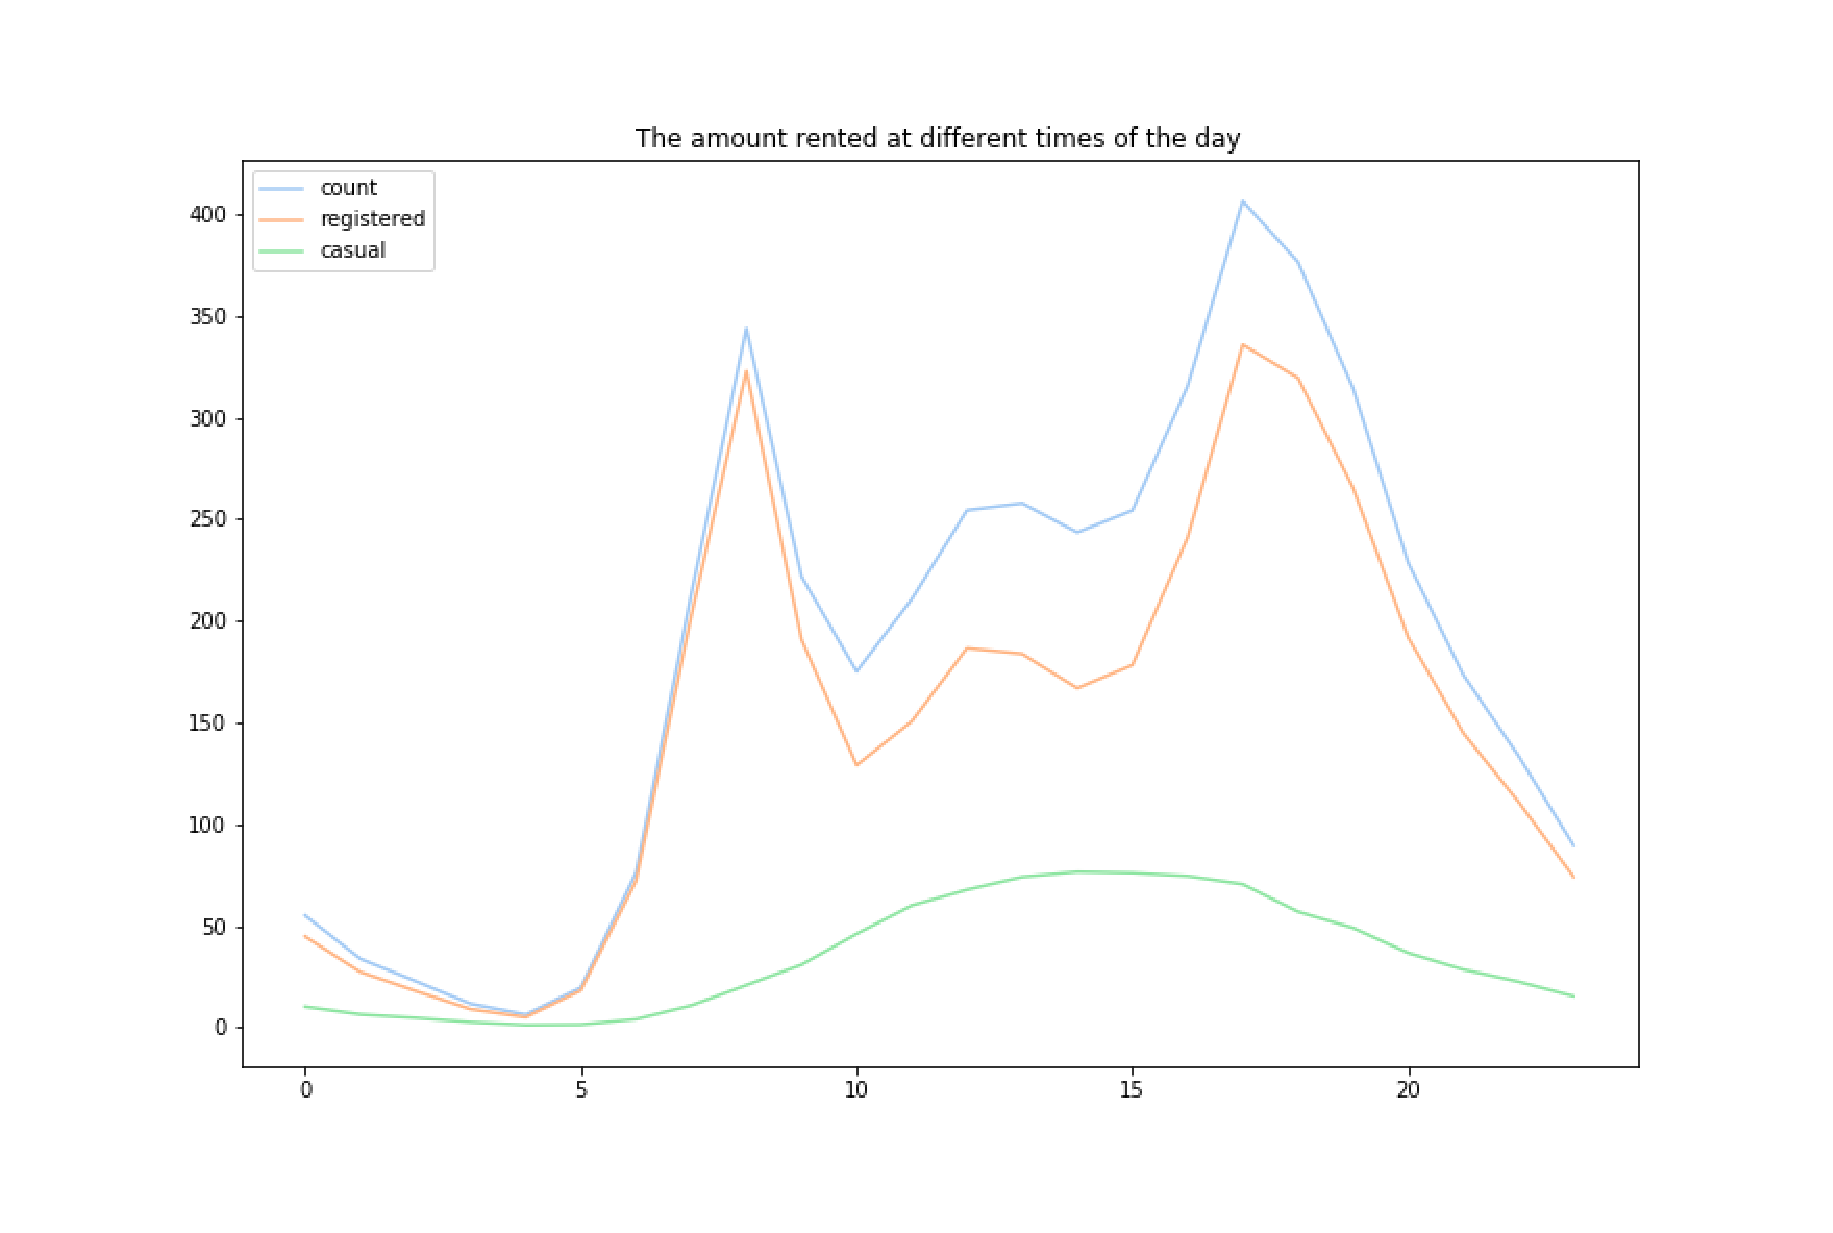
\includegraphics[width=0.8\textwidth]{figures//Time_trends_day.eps}\\
\caption{The amount rented at different times of the day} \label{framework}
\end{figure}




\section{Feature Selection and Feature Importance} \label{sec-feature}

\begin{itemize}
  \item
  The influence of characteristics on count is as follows:\\
  hour>temp>atemp>humidity>month>season>year>weather\\
  >windspeed>workingday>weekday>day>holiday
  \end{itemize}
  \begin{figure}
  \centering
  \selectcolormodel{rgb}
  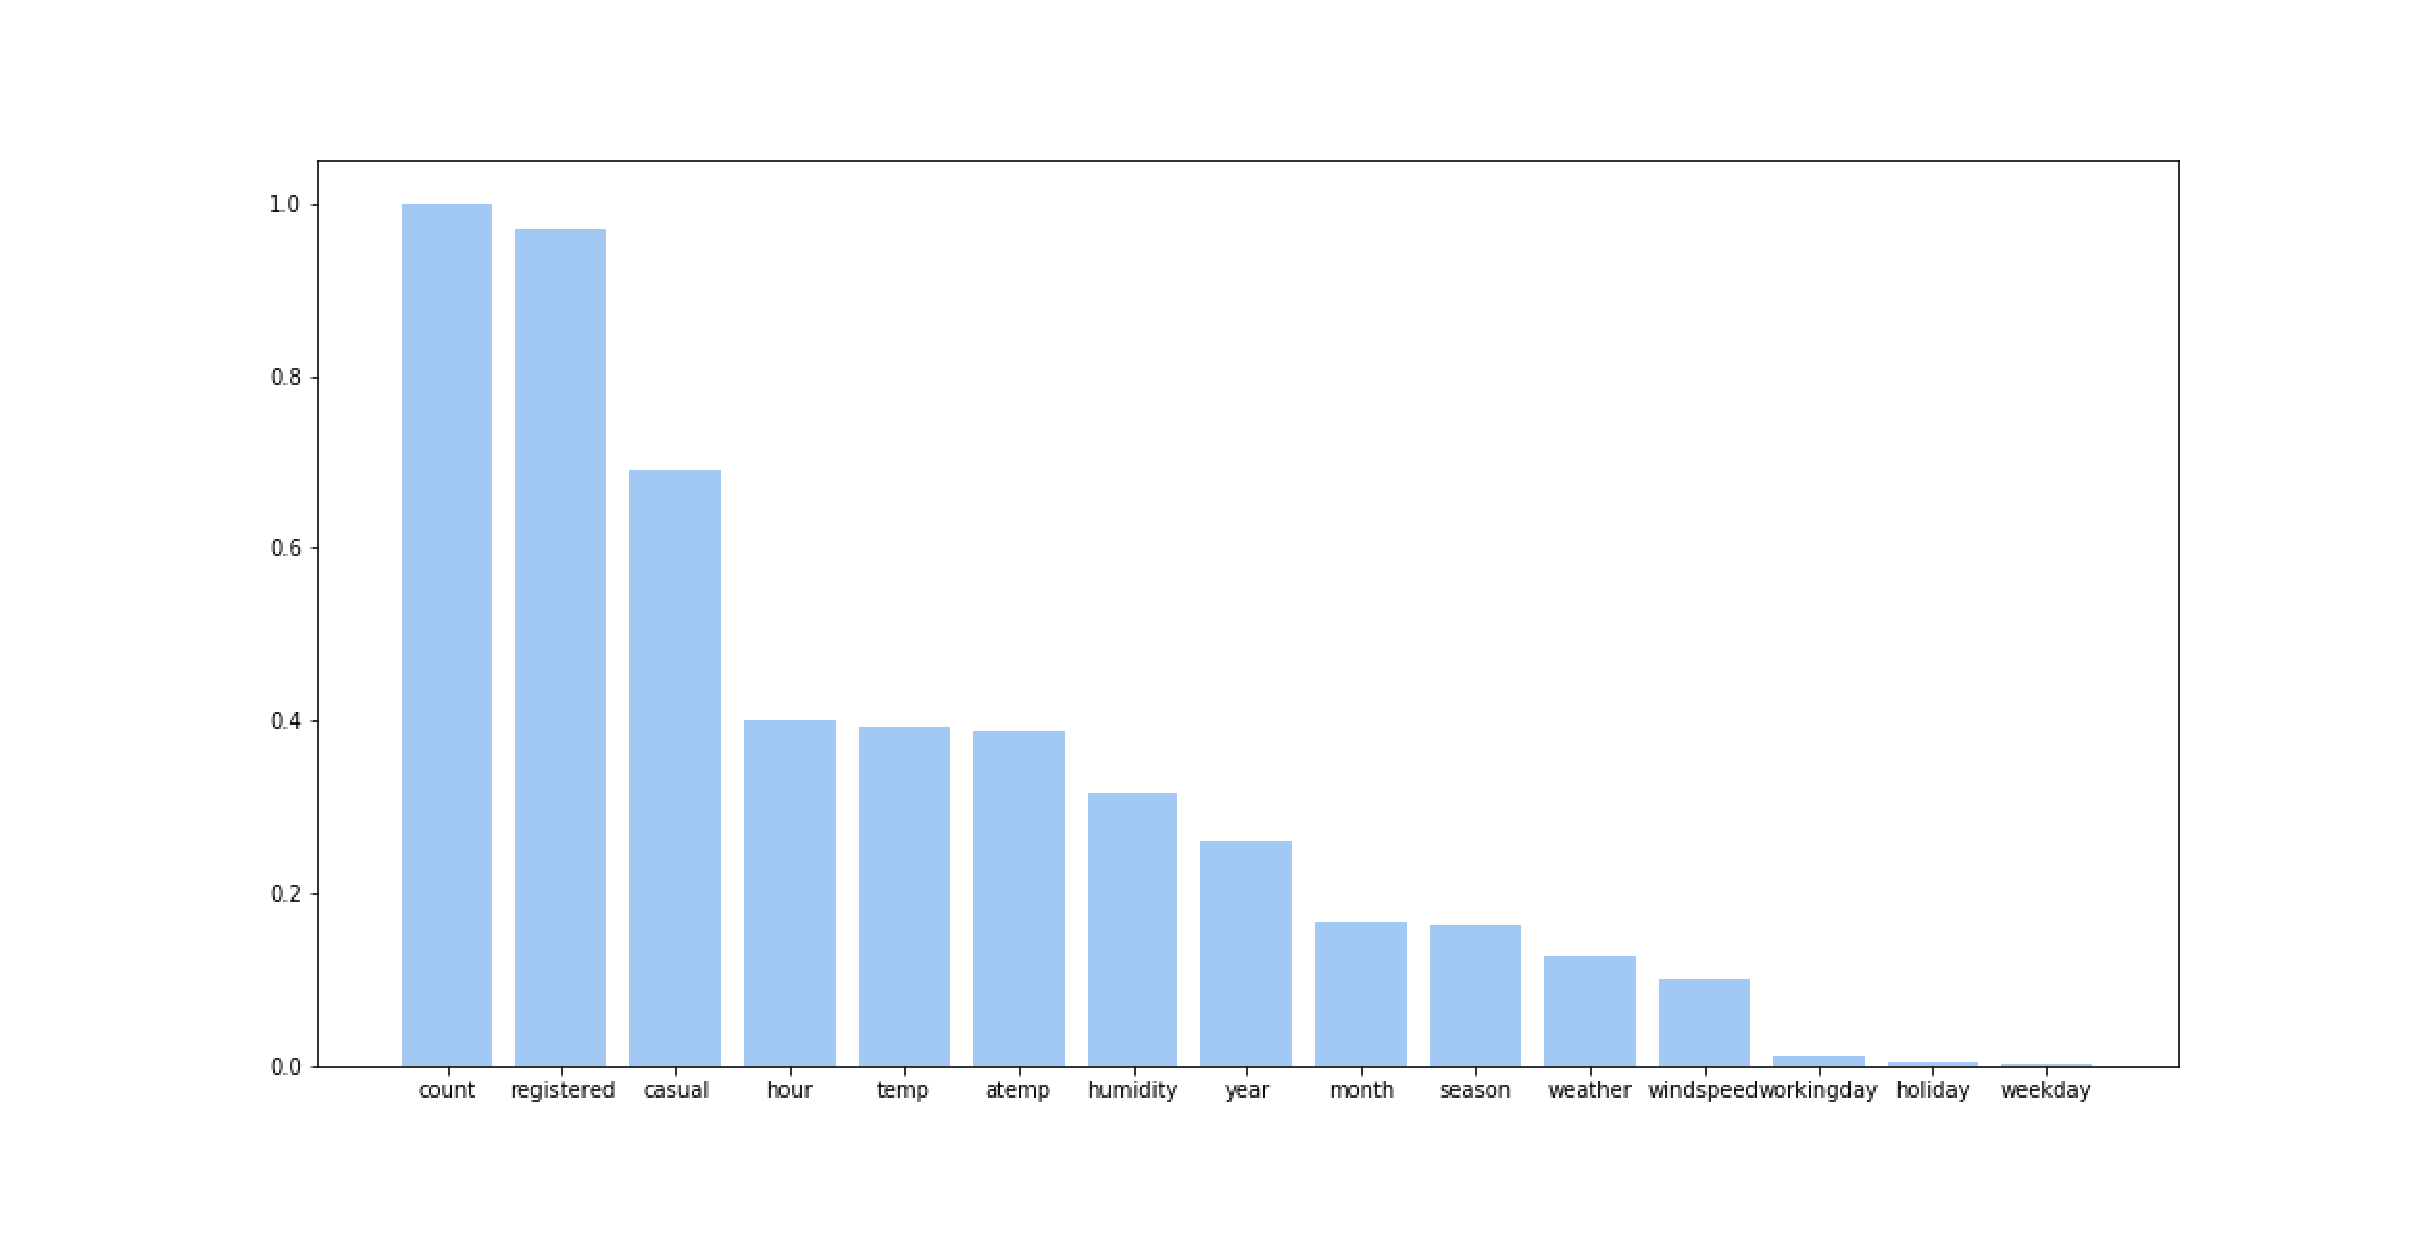
\includegraphics[width=0.8\textwidth]{figures//cor_rank.eps}\\
  \caption{Correlation rank} \label{framework}
\end{figure}
\begin{itemize}
  \item
  Weather characteristics analysis
\end{itemize}
  \begin{figure}
  \centering
  \selectcolormodel{rgb}
  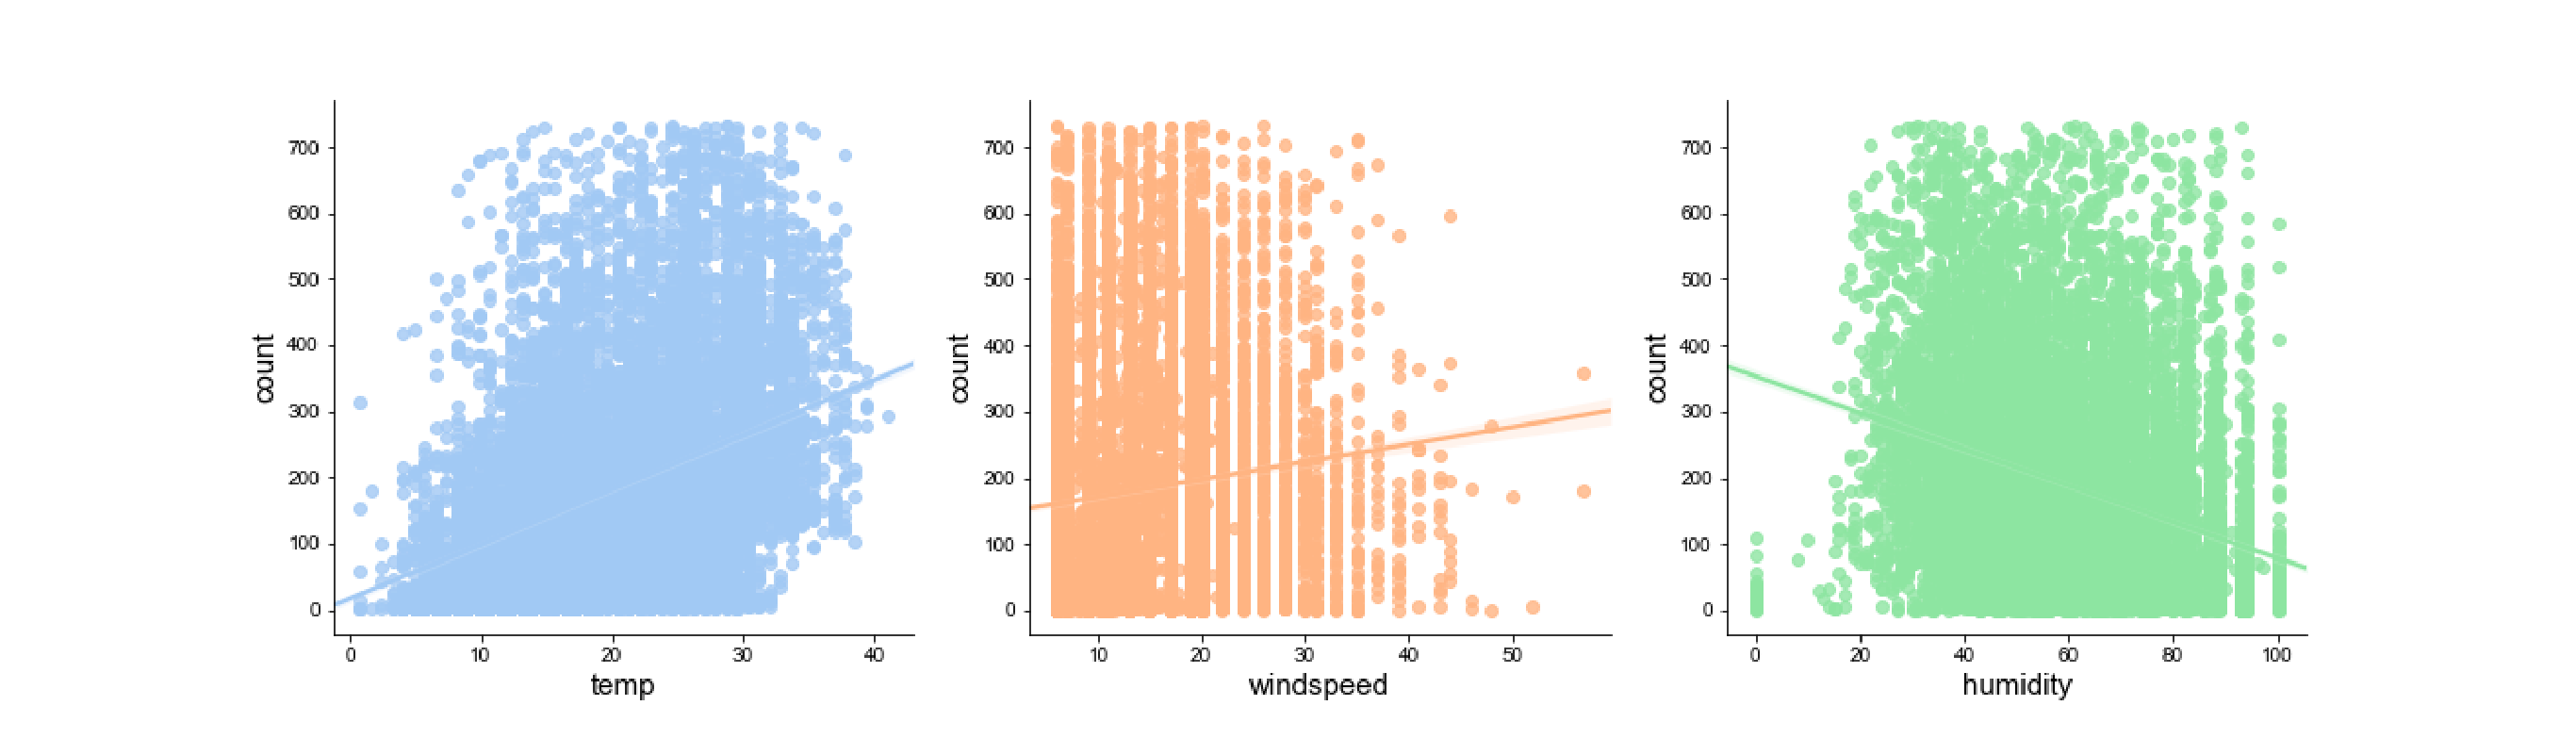
\includegraphics[width=0.8\textwidth]{figures//weather.eps}\\
  \caption{The effect of weather on rental amount} \label{framework}
\end{figure}        


\section{Modeling and Result}\label{sec-result}

\begin{itemize}
  	\item[Model:] RandomForestRegressor
    
\end{itemize}
\begin{tabular}{ c | c | c  }
    \toprule
    Result     &  The initial model    & After cross validation       \\
    \midrule
    Accuracy       &  0.9338   &  0.9249       \\

    MSLE      &  0.0152   &  0.0159     \\

     
    \bottomrule
\end{tabular}



\section{Conclusion}\label{sec-conclusions}

\begin{itemize}
  \item
    Cross-validation by grid search did not decrease the RMSE of the model and did not improve the accuracy of the model.
  The effect did not come up to expectations.
  \item
  The limitation of this study is that it does not consider whether there is overfitting of the model, and further experiments can be carried out in future studies.
\end{itemize}




